%здесь нужно будет куски текста и картинки  из двух статей перевести. Ссылки нужно будет добавить - их нет в зотеро многих. В описании картинок - не забывать добавить из какой они статьи - ссылку.
%materials/part6_2_nucl_pol/pnas2015 и nar2014

\subsection{Введение}
%2S pnas2015 - желтое выделение.
    Транскрипция РНК-полимеразы II (Pol II) индуцирует обширное ремоделирование хроматина, сопровождающееся ковалентными модификациями гистонов и их обменом (см. напр. \cite{smolle_resetting_2013,das_histone_2013,zentner_regulation_2013}). В то же время, гистоны вытесняются только из высокотранскрибируемых генов \cite{kristjuhan_evidence_2004,schwabish_evidence_2004,lee_evidence_2004}; таким образом, Pol II обычно встречается с нуклеосомами во время транскрипции каждого участка ДНК длиной $\sim$200 пар оснований. Остающиеся нуклеосомы на транскрибируемых генах образуют два типа барьеров для транскрипции Pol II \cite{das_histone_2013,weber_nucleosomes_2014}. Во-первых, каждая нуклеосома представляет собой барьер, на котором Pol II приостанавливается после транскрипции 40–50 п.н. от границы нуклеосомы проксимальной к промотор. Во-вторых, намного выше барьер образован первой (+1) транскрибированной нуклеосомой, по крайней мере в дрозофилы \cite{weber_nucleosomes_2014}; в этом случае Pol II останавливается на нуклеосомной границе. Остановившаяся Pol II обнаружена на многих генах: от 15\% до более чем 50\% генов у мух и человека соответственно \cite{guenther_chromatin_2007,muse_rna_2007,zeitlinger_rna_2007}. В во многих случаях остановившаяся Pol II была картирована вместе с хорошо расположенной +1 нуклеосомой. Предполагается, что эта +1 нуклеосома может через паузирование влиять на общий уровень экспрессии генов \cite{weber_nucleosomes_2014,mavrich_nucleosome_2008}. 
    
    Данные \textit{in vitro} экспериментов установили, что даже одна нуклеосома может образовывать высокий барьер первого типа для транскрипции Pol II \cite{brown_activator-dependent_1996,izban_transcription_1991,bondarenko_nucleosomes_2006,kireeva_nature_2005,kulaeva_mechanism_2009,hall_high_2009} и что факторы транскрипции, шапероны гистонов, модификации гистонов и т.д. необходимы Pol II  для преодоления этого барьера \cite{bondarenko_nucleosomes_2006,kireeva_nature_2005,brown_disruption_1997,izban_factor-stimulated_1992,hsieh_histone_2013,kulaeva_rna_2010,kim_human_2010,guermah_synergistic_2006,carey_rsc_2006,bintu_nucleosomal_2012,jin_synergistic_2010}. Сильный барьер образуется после транскрипции 40–50 п.н. за границей нуклеосомы [область +(40–50)], является нуклеосомно-специфичным, специфичным для Pol II и был описан для всех проанализированных организмов, от дрожжей до человека \cite{izban_transcription_1991,bondarenko_nucleosomes_2006,kireeva_nature_2005}. Таким образом +40–50 нуклеосомный барьер является ``универсальным'' признаком транскрипции через хроматин с помощью Pol II и может использоваться для регуляции экспрессии на уровне элонгации транскрипта \cite{bondarenko_nucleosomes_2006}. На любой последовательности ДНК, барьер формируется в различных положениях внутри региона +(40–50)  \cite{bondarenko_nucleosomes_2006}.

\subsection{Создание моделей комплекса в положении активного центра +49 (нулевая петля)}
%2S дать желтый текст из nar2014, картинки основного текста и таблицу тоже
    Наши предыдущие исследования выявили элонгационный комплекс +49 (ЭК+49, 49 п.н. от промотор-проксимальной границы нуклеосомы), содержащий нулевую петлю, в качестве ключевого интермедиата, который помогает нуклеосомам выживать во время транскрипции \cite{kulaeva_mechanism_2009}. В данной работе мы смоделировали комплекс ЭК+49 путем докирования структуры высокого разрешения элонгационного комплекса дрожжевой полимеразы II  на нуклеосому с 601 хорошо позиционирующей последовательностью ДНК \cite{vasudevan_crystal_2010,kettenberger_complete_2004} (Рисунок \ref{fig:p6_2_n2014_f1}).
    
    ЭК+49 имеет следующие свойства (Рисунок \ref{fig:p6_2_n2014_f1}): (i) Основная часть молекулы Pol II обращена в раствор и не имеет стерических конфликтов с гистонами нуклеосомного кора, (ii) Изгиб ДНК на $90^{\circ}$, присутствующий в ЭК, обращен к октамеру и позволяет формировать нулевую петлю, (iii) контакты ДНК-гистоны на участком ДНК длиной $\sim$20 п.н. за ЭК стабилизируют нулевую петлю, (iv) вытеснение 50 п.н. с конца нуклеосомы дистального к промотору снижает размер области ДНК, взаимодействующей с гистонами перед ферментом с $\sim$100 до $\leq$50 п.н. Это, вероятно, способствует дальнейшему разворачиванию ДНК с октамера впереди от Pol II и транскрипции через нуклеосому \cite{kulaeva_mechanism_2009}. (v) Отрицательно заряженная область на поверхности Pol II (предполагаемая последовательность, стабилизирующая нулевую петлю, область ZLS - zero-loop-stabilizing sequence) находится в непосредственной близости к положительно заряженной области октамера гистонов и, таким образом, может стабилизировать нулевую-петлю и способствовать выживанию нуклеосом во время транскрипции.
    
\subsection{Выявление отрицательно заряженных регионов на предполагаемых
гистон-взаимодействующих поверхностях Pol II}
    
    Используя модель ЭК+49 (рис. \ref{fig:p6_2_n2014_f1}), были идентифицированы предполагаемая взаимодействующая с Pol II поверхность на октамере гистонов и три взаимодействующие с гистоном поверхности Pol II (рис. \ref{fig:p6_2_n2014_f2}A). Все взаимодействующие с гистонами поверхности заряжены отрицательно и локализуется на самой крупной субъединице дрожжевой Pol II (yRpb1, регионы 1–3, рис. \ref{fig:p6_2_n2014_f2}А). Для дальнейшей оценки возможной роли предполагаемых областей ZLS на Pol II во время транскрипции через хроматин было оценено их присутствие и сохранение в различных структурно связанных эукариотических и прокариотические РНК-полимеразах  (Таблица \ref{tab:p6_n2014_t1}). РНКП \textit{Escherichia coli}, которая использует механизм транскрипции типа Pol II через хроматин \cite{walter_bacterial_2003} не была включен в это исследование, потому что структуры с высоким разрешением этого фермента пока не получена. Последовательности областей 2 и 3 ZLS является консервативными с более, чем 50\% идентичностью, у мультисубъединичных прокариотических РНКП \textit{T. thermophilus} и \textit{T. aquaticus} ( структурно сходных с Pol II \cite{vassylyev_structural_2007,zhang_crystal_1999}), а как область 1 консервативна только в эукариотических РНКП. Гомологичных последовательностей в односубъединичный РНКП бактериофага Т7 не было обнаружено.
    
    Предполагается, чтобы чистый отрицательный заряд последовательности ZLS может быть важен для стабилизации нулевой петли и эффективного выживания нуклеосомы в ходе транскрипции \cite{kulaeva_mechanism_2009}. В соответствии с этим предположением области ZLS отрицательно заряжены в дрожжевой Pol II (Рисунок \ref{fig:p6_2_n2014_f2}A), которая не смещает нуклеосомы во время транскрипция \cite{kireeva_nucleosome_2002,walter_bacterial_2003}. Области ZLS Pol II человека также отрицательно заряжены, и поэтому ожидается, что Pol II человека также сохраняет нуклеосомную структуры во время транскрипции. Это предложение согласуется с наблюдаемыми сходными паттернами сильной нуклеосомной паузы, которые характерны для Pol II человека и дрожжей \cite{bondarenko_nucleosomes_2006}.
    
    Напротив, отрицательные заряды областей ZLS не сохранились в других проанализированных прокариотических РНКП (из \textit{T. thermophilus} и \textit{T. aquaticus}) (Рисунок \ref{fig:p6_2_n2014_f2}Б и Таблица \ref{tab:p6_n2014_t1}).
    
    Хотя предполагаемая взаимодействующая с гистонами поверхность РНКП \textit{T. thermophilus}  имеет некоторые регионы с локальным отрицательным зарядом (рис. \ref{fig:p6_2_n2014_f2}Б), в данном регионе нет суммарного положительного заряда. Данные показывают, что чистый отрицательный заряд внутри взаимодействующего с гистоном поверхности этих РНКП положительно коррелирует с вероятность выживания нуклеосом при транскрипции. Кроме того, расстояние между областями ZLS и поверхность октамера гистонов в среднем на $\sim$5\AA больше для РНКП \textit{T. thermophilus}, чем у дрожжевой Pol II. Более низкий полный отрицательный заряд областей ZLS и больше расстояние между РНКП и октамером гистонов, вероятно, уменьшает силу взаимодействия между РНКП и гистонами. Соответственно, РНКП, которые имеют более низкий полный отрицательный заряд области ZLS, как ожидается, формируют менее стабильный комплекс нулевой петли в положении ЭК +49. Поскольку стабильная нулевая петля, вероятно, необходима для выживания нуклеосом, ожидается, что эффективность выживаемости будет ниже во время транскрипции РНКП \textit{T. thermophilus} и \textit{T. aquaticus} по сравнению с Pol II. Поскольку стабильная нулевая петля также приводит нуклеосомной паузе в области +45 \cite{hsieh_histone_2010}, уменьшение паузирования в положении +45 также ожидается во время транскрипции этими РНКП. Чтобы проверить эти предсказания модели, эксперименты по транскрипции на идентичных ДНК и нуклеосомных матрицах были проведены с помощью РНКП \textit{T. thermophilus} и \textit{T. aquaticus}.
    
\begin{figure} [H]
    \centering
    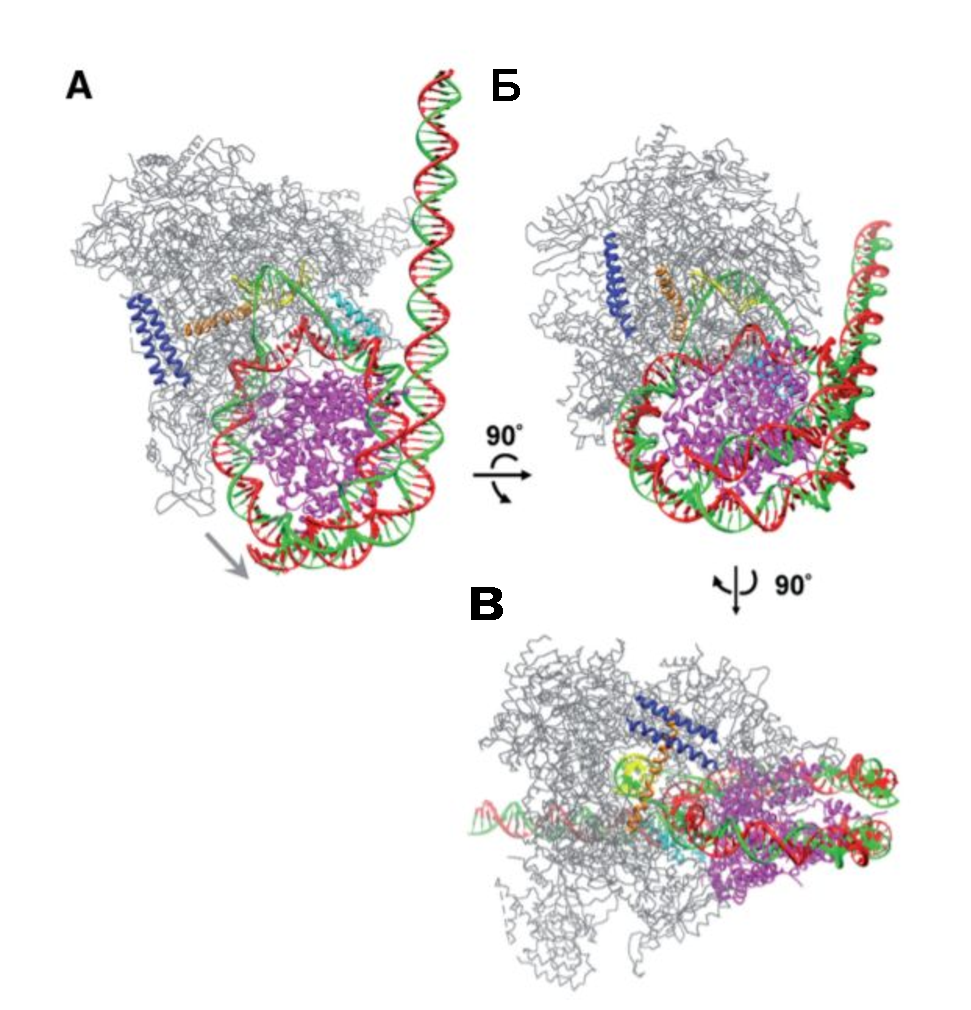
\includegraphics{images/p6/p6_2/p6_2_nar2014_f1.pdf}
    \caption[Модель ЭК+49 (нулевая петля) с дрожжевой Pol II]{Модель ЭК+49 (нулевая петля) с дрожжевой Pol II. (A) Структуры нуклеосомы и комплекса элонгации Pol II дрожжей с активным сайтом в позиции +49 [PDB 3LZ0 и 1Y1W соответственно \cite{vasudevan_crystal_2010,kettenberger_complete_2004}] были объединены с использованием подхода докинга. Чтобы позволить формирование небольшой внутринуклеосомной петли ДНК, содержащей транскрибирующую Pol II, промотор-дистальная область нуклеосомной ДНК длиной 50 п.н. была отмотана от октамера \cite{kulaeva_mechanism_2009}. Октамер нуклеосомы изображен пурпурным. Матричная цепь ДНК, нематричная цепь ДНК и цепи РНК изображены зеленым, красным и желтым, соответственно. Мостовая спираль (bridge), зажим (clamp), C-терминальная двойная спираль (coiled coil) и остальная часть молекулы Pol II показаны оранжевым, голубым, синим и серым, соответственно. Серая стрелка указывает направление транскрипции. (Б) Структура была повернута на $\sim 90^{\circ}$ вокруг горизонтальной оси. (В) Затем структура была повернута на 90 $^{\circ}$ вокруг вертикальной оси.}
    \label{fig:p6_2_n2014_f1}
\end{figure}
   
\begin{figure} [H]
    \centering
    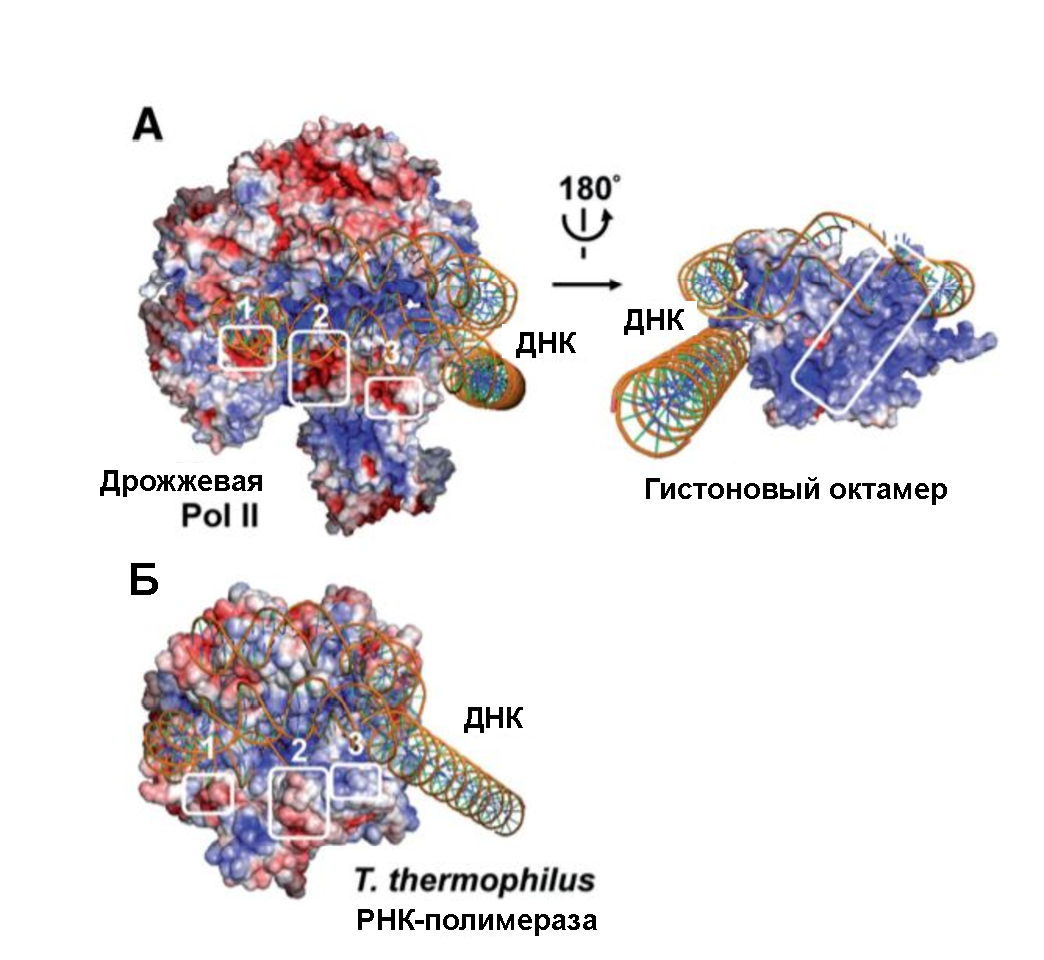
\includegraphics{images/p6/p6_2/p6_2_nar2014_f2.pdf}
    \caption[Отрицательно заряженная поверхность Pol II может стабилизировать интермедиат нулевой петли посредством взаимодействия с гистоновым октамером]{Отрицательно заряженная поверхность Pol II может стабилизировать интермедиат нулевой петли посредством взаимодействия с гистоновым октамером. (А) Предполагаемые взаимодействующие с гистонами молекулярные поверхности дрожжевой Pol II. Слева: Три идентифицированные поверхности на большой субъединице Rpb1 дрожжевой Pol II внутри ЭК+49 (смоделирована как на Рисунке \ref{fig:p6_2_n2014_f1}), взаимодействующие с октамером гистонов (не показан), показаны белыми квадратами (области 1–3). Справа: контактирующая поверхность на октамере гистонов (повернут на $180^{\circ}$ вокруг вертикальной оси). Самый темный синий и самый темный красный цвет обозначает электростатический потенциал 5 кТ/е и -5 кТл/е, соответственно. ДНК показана желтым. (Б) Молекулярные поверхности РНКП \textit{T. thermophilus} (PDB ID 2O5I) в гипотетической модели комплекса ЭК+49 окрашены по величине электростатического потенциала (октамер гистонов не показан). Области 1–3 гомологичны контактирующим с гистоном поверхностям Pol II (Figure \ref{fig:p6_2_n2014_f2}A).}
    \label{fig:p6_2_n2014_f2}
\end{figure}

\begin{table}
\begin{threeparttable} [h!]
    \centering
    \begin{tabularx}{\textwidth}{|X|X|X|X|X|X|}
\hline
        Фермент & Виды & Заряд ZLS области\tnote{a} & Нулевая петля при +49 & Высота +45 барьера & Выживание нуклеосом \\
\hline
        Pol II (RPB1) & \textit{H. sapiens} & -8 & ND & $+++++$\tnote{b} & ND \\
        Pol II (Rpb1) & \textit{S. cerevisiae} & -15 & $+$\tnote{c} & $+++++$\tnote{b} & $+++++$\tnote{d} \\
        РНКП ($\beta'$) & \textit{T. thermophilus} & +1 & ND & $+$\tnote{e} & ND \\
        РНКП ($\beta'$) & \textit{T. aquaticus} & +1 & $-$\tnote{e} & $+$\tnote{e} & - \\

\hline
    \end{tabularx}
\begin{tablenotes}
    \item[a] Полные заряд гомологичной области 1434–1450 ZLS субъединицы Rpb1 дрожжевой Pol II.
    \item[b]  Ссылка \cite{bondarenko_nucleosomes_2006}.
    \item[c]  Ссылка \cite{kulaeva_mechanism_2009}.
    \item[d]  Ссылка \cite{walter_bacterial_2003}.
    \item[t]  Эта работа.
     
   \end{tablenotes}
\end{threeparttable}
    \caption{Корреляция между присутствием отрицательно заряженных областей на обращенной к октамеру поверхности РНКП, высотой нуклеосомного барьера и выживаемостью нуклеосом во время транскрипции}
    \label{tab:p6_n2014_t1}
\end{table}

\subsection{Более высокий отрицательный заряд области ZLS коррелирует с более сильным барьером +45 и более эффективной выживаемостью нуклеосом при транскрипции}
    
    Данные о чистом заряде региона ZLS, силе барьера +45 нуклеосомного паузирования и судьбы нуклеосом во время транскрипции различными РНКП просуммирована в Таблице \ref{tab:p6_n2014_t1}. Наличие более высокого отрицательного заряда область ZLS положительно коррелирует с формированием ключевого промежуточного продукта, который сильно способствует выживанию нуклеосом (нулевая петля в положении +49), с более сильным паузированием в области +45 и более эффективным выживанием нуклеосом во время транскрипции.
    
    В целом данные свидетельствуют о том, что присутствие и полный заряд области ZLS частично определяет структуру ключевого интермедиата, сформированного в позиции +49, а в в свою очередь, судьбу нуклеосом при транскрипции. Когда ZLS область присутствует и отрицательно заряжена (например, у Pol II человка или дрожжей), нуклеосомное паузирование в положении +45 является сильным, нулевая петля образуется в положении +49 и нуклеосомы эффективно выживают во время транскрипции. Когда регион ZLS присутствует, но не содержит отрицательного заряда (например, в РНКП \textit{T. thermophilus} и \textit{T. aquaticus}), нуклеосомная пауза в +45 положении слабая, нулевая петля не образуется, и нуклеосомы теряются во время транскрипции.
    
    
    
\subsubsection{Дискуссия и сравнение с экспериментами} %not edited
%2S дать фиолетовый текст из nar2014, картинки основного текста
    
    В нашей работе роль отрицательно заряженной области на поверхности Pol II (области ZLS) во время транскрипции через хроматин было оценено с использованием компьютерного моделирования и экспериментального анализа механизма транскрипция через хроматин различными РНКП. Вычислительное моделирование показало, что в комплексе элонгации, определяющем выживаемость нуклеосом во время транскрипции (ЭК+49), три области ZLS находятся в непосредственной близости к положительно заряженной области октамера гистонов и таким образом могут стабилизировать нулевую-петлю и облегчать нуклеосомную выживаемость при транскрипции (рисунки \ref{fig:p6_2_n2014_f1} и \ref{fig:p6_2_n2014_f2}). Анализ транскрипции РНКП \textit{T. thermophilus} и \textit{T. aquaticus}, у которых есть незаряженные области ZLS, предполагает, что в этом случае нуклеосомная пауза +45 слабая, нулевая-петля не образуется, и нуклеосомы теряются во время транскрипции. Напротив, транскрипция Pol II, имеющая отрицательно заряженные области ZLS, приводит к сильной нуклеосомной паузе в +45 положении, образовании нулевой-петли и выживаемости нуклеосом \cite{kireeva_nucleosome_2002,kulaeva_mechanism_2009,bondarenko_nucleosomes_2006}. Сила +45 паузы частично определяется отрицательным зарядом в области ZLS Pol II. Таким образом свойства (в частности, заряд) области ZLS диктуют все ключевые параметры механизма транскрипции через нуклеосому.
    
    Как может наличие и заряд ZLS региона влиять на эти множественные аспекты транскрипции через хроматин? Ранее мы предположили, чтобы регион ZLS может влиять на структуру/стабильность ключевого интермедиата, содержащего нулевую-петлю (ЭК+49), образующегося во время транскрипции через нуклеосому \cite{kulaeva_mechanism_2009}. Это промежуточное состояние, в свою очередь, как ожидалось будет играть связывающую роль между паузированием в +45 положении и эффективным выживанием нуклеосом во время транскрипции \cite{hsieh_histone_2010}. В соответствии с этим предположением наши текущие данные свидетельствуют в пользу того, что РНКП у которых отсутствует заряд в области ZLS или сама область не сталкиваются с сильным нуклеосомным барьером, не образуют нулевые-петли и не могут поддерживать эффективное выживание нуклеосом.
    
    Основываясь на наших данных, мы предлагаем следующую модель, объясняющую наблюдаемую связь между +45 паузой, образование нулевой петли и судьбой нуклеосом. По мере того как разные РНКП входят в нуклеосому и подходят к области +45 (комплекс 1), они образуют нулевую-петлю с разной эффективностью. В частности, дрожжевой Pol II образует нулевую петлю (комплекс 2) с высокой эффективностью \cite{kulaeva_mechanism_2009}, отчасти потому, что ее ZLS-область заряжена отрицательно и стабилизирует нулевую петлю за счет взаимодействия с положительно заряженной поверхностью октамера гистонов. Формирование нулевой петли вызывает медленное раскручивание ДНК перед ферментом (комплекс 3) - то есть сопровождается сильной нуклеосомной паузой. ДНК позади РНКП повторно оборачивается вокруг октамера гистонов и нуклеосома восстанавливается в исходном положении \cite{kulaeva_mechanism_2009}. Напротив, во время транскрипции РНКП \textit{T. thermophilus} и \textit{T. aquaticus} с незаряженными ZLS областями нуклевая петля (если образуется) нестабильна (комплекс 2'). Таким образом, транскрипция сопровождается лишь незначительной нуклеосомной паузой и смещением гистонового октамера при дальнейшей транскрипции через нуклеосому \cite{walz_sequence_1975}. Таким образом, структуры ключевых промежуточных продуктов образующиеся во время транскрипции через +45 область нуклеосомной ДНК, вероятно, обуславливают множество аспектов транскрипции через хроматин, включая нуклеосомную паузу и судьбу гистонов при транскрипции. Присутствие и заряд региона ZLS вряд ли будет единственным фактором, влияющим на результат транскрипции через хроматин. Таким образом, расстояние между областями ZLS и октамером гистонов в ЭК+49, вероятно, важно для стабильность нулевой петли.
    
    Отрицательно заряженная область 2 ZLS дрожжевого Pol II  локализована в свитч-2 домене и, вероятно, важна для разделения нитей ДНК при транскрипции \cite{kettenberger_complete_2004}. Она также локализована в кислотном домене, который влияет на активацию транскрипции, активность Pol II дрожжей и важен для нормального роста клеток \cite{xiao_highly_1994}. Наши исследования предполагают дополнительную важную функцию области 2 ZLS - определение скорости прохождения РНКП через нуклеосому и судьбу нуклеосом при транскрипции в хроматине. Эта функция особенно важна для эукариотических Pol II: в данном случае консервативный отрицательно заряженная область ZLS, скорее всего, способствует выживанию нуклеосом и поддержанию гистоновых меток во время транскрипции.
    
% \begin{figure} [H]
%     \centering
%     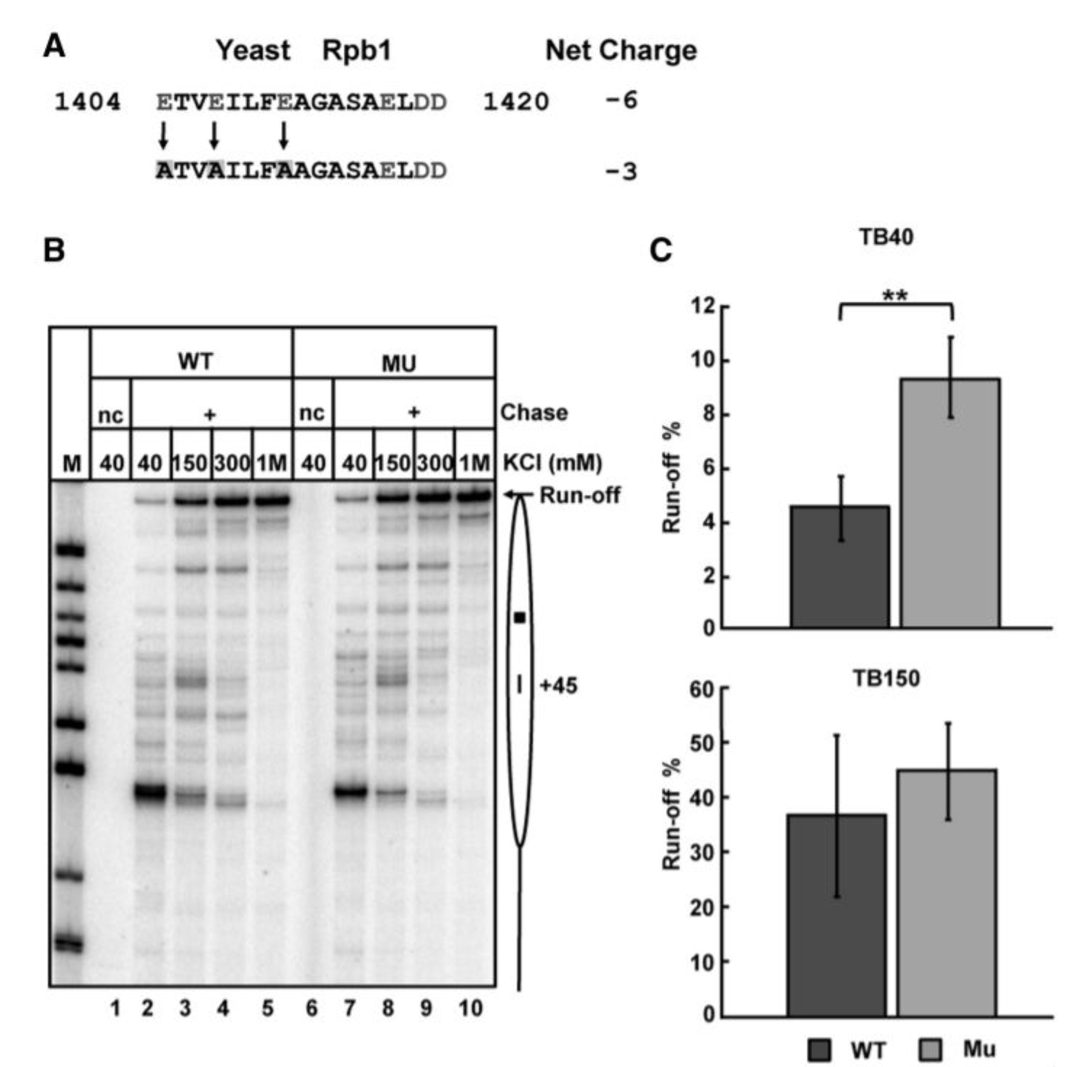
\includegraphics{images/p6/p6_2/p6_2_nar2014_f6.pdf}
%     \caption{MU Pol II, имеющий более низкий отрицательный заряд взаимодействующей с гистонами поверхности, встречает более низкий нуклеосомный барьер. (A) Стратегия Pol II мутагенез. Три аминокислоты Glu субъединицы yRpb1 в положениях 1404, 1407 и 1411 одновременно были преобразованы в Ala (отмечены желтым квадратов), изменяя чистый заряд области 2 ZLS с –6 до –3. Отрицательно заряженные аминокислоты выделены жирным красным цветом. (Б) Транскрипция 603 нуклеосомные матрицы с помощью WT и MU yPol II при указанных концентрациях KCl. nc означает отсутствие погони. РНК с импульсной меткой анализировали с помощью денатурирующий PAGE. Другие обозначения такие же, как на рисунке \ref{fig:p6_2_n2014_f4}. (В) Количественное определение транскриптов, полученных при 40 мМ KCl и 150 мМ KCl WT. или Mu yPol II (Рисунок \ref{fig:p6_2_n2014_f7}Б). Показаны средние значения из трех экспериментов и стандартные отклонения (** означает значение P <0,01).}
%     \label{fig:p6_2_n2014_f6}
% \end{figure}
    
\begin{figure} [H]
    \centering
    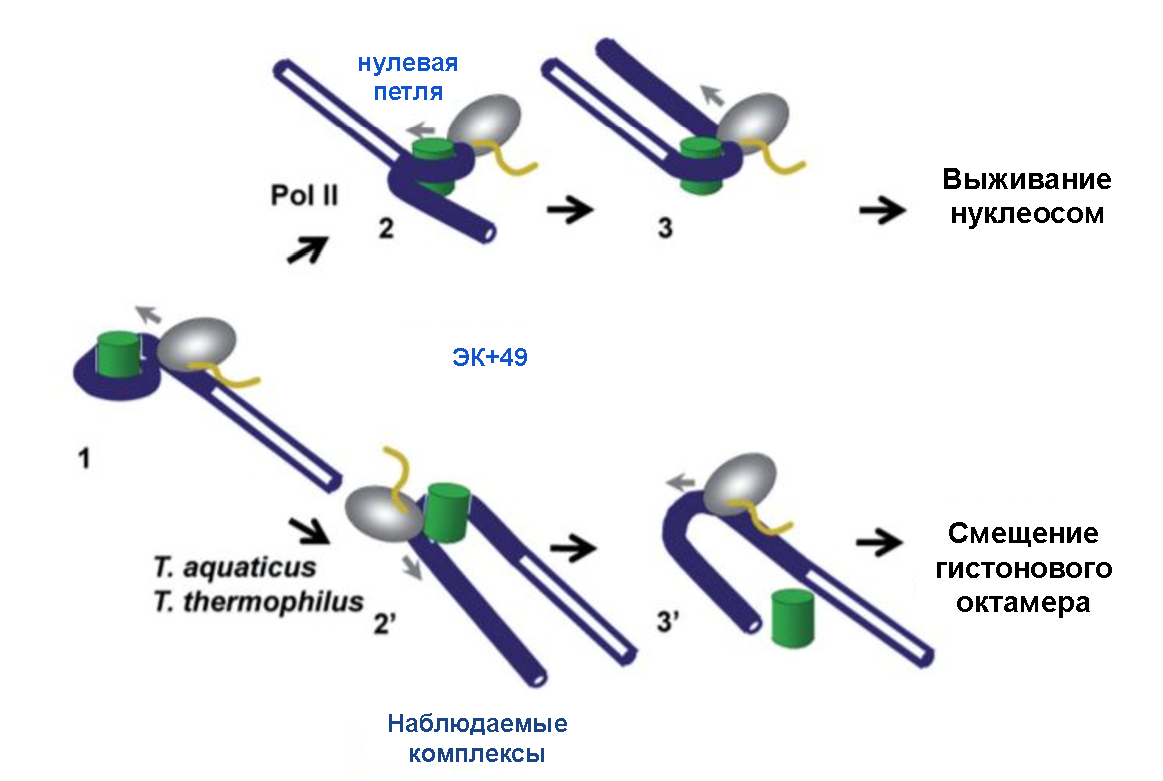
\includegraphics[width=\textwidth]{images/p6/p6_2/p6_2_nar2014_f7.pdf}
    \caption[Предлагаемые механизмы транскрипции через нуклеосому разными РНКП.]{Предлагаемые механизмы транскрипции через нуклеосому разными РНКП. Мы предлагаем, чтобы общий отрицательный заряд на поверхность РНКП, которая обращена к октамеру гистонов, частично обуславливает структуру важного промежуточного комплекса (ЭК+49). Более подробное описание см. в тексте.}
    \label{fig:p6_2_n2014_f7}
\end{figure}
    
    
    
    
    
    
    
    
    
    
\subsubsection{Методы}
%2S зеленый кусок текста из nar2014
\subsubsection{Моделирование Pol II в позиции +49 в нуклеосоме и анализ структурных особенностей моделируемых комплексов}
    
    Модель была построена с использованием программа UCSF Chimera (\url{http://www.cgl.ucsf.edu/chimera/}) \cite{pettersen_ucsf_2004} за счет объединения структуры коровой частицы нуклеосомы на основе 601 последовательности [PDB ID 3LZ0 \cite{vasudevan_crystal_2010}] со структурой элонгационного комплекса дрожжей Pol II [PDB ID 1Y1W \cite{kettenberger_complete_2004}]. Веб-сервер 3D-DART использовался для восстановления конформации ДНК \cite{van_dijk_3d-dart_2009}. Остальные подходы следовали описанию в опубликованной статье \cite{kulaeva_mechanism_2009}. ЭК+49 \textit{T. thermophilus} был построен путем наложения кристаллической структуры РНКП [PDB ID: 2O5I \cite{vassylyev_structural_2007}] на модель Pol II ЭК+ 49. Молекулярные электростатические поверхности белков рассчитывали с помощью APBS \cite{baker_electrostatics_2001} и отображали с помощью PyMOL (\url{http://www.pymol.org}). Расстояния между отрицательно заряженной поверхность Pol II и октамером гистонов, а также вовлеченные аминокислотные остатки также были идентифицированы в PyMOL. Все белковые последовательности РНКП в этой статьи были взяты из базы данные RefSeq NCBI (NP\_000928.1, NP\_010141.1, NP\_418415.1, YP\_145078.1 и CAB65466.3) (\url{http://www.ncbi.nlm.nih.gov/guide/}). Последователности различных РНКП были выровнены с помощью NCBI Blast (\url{http://blast.ncbi.nlm.nih.gov}).
    
    











\subsection{Создание моделей комплекса полимеразы и нуклеосомы в положении активного центра +42}
%2S pnas2015 - зеленый текст
%(картинки только основные, не сапплемент, кроме s5 и s8 - которые нужно дать.)
%дать синий текст
\subsubsection{Экспериментальные данные}
    Эксперименты проводились с использованием мононуклеосомных матриц, которые повторяют многие важные аспекты транскрипции PolII в хроматине \textit{in vivo} \cite{kulaeva_rna_2010,kireeva_nucleosome_2002,hsieh_histone_2010}. Механизм образования нуклеосомного барьера при транскрипции изучен с использованием 601 и 603 мононуклеосом, которые содержат ДНК последовательность с полярным барьером для транскрипции  (PBS) и образуют очень сильный нуклеосомный барьер в одна из двух транскрипционных ориентаций (непермиссивная ориентация) \cite{bondarenko_nucleosomes_2006,kulaeva_mechanism_2009,gaykalova_polar_2011}. Матрицы ДНК были разработаны так, чтобы Pol II останавливалась в положениях -41 и -5 (на 41 или 5 п.н. выше промоторно-проксимальной границы нуклеосомы) при наличие различных частичных комбинаций нуклеотид трифосфатов. Pol II спонтанно останавливается во время транскрипции непермиссивной нуклеосомы 601 при 150 мМ KCl на +46 и +48 позиции. Остановка обратима, так как Pol II может транскрибировать всю матрицу после дестабилизации гистонового октамера в 1M KCl.
    
    Состояние Pol II после встречи с высоким нуклеосомный барьером изучалось с помощью 601-ой ДНК матрицы, которая представляет собой самый сильный нуклеосомный барьер для транскрипции Pol II \cite{bondarenko_nucleosomes_2006}. Pol II был спонтанно останавливалась в позиции +46 и +48 на 601-нуклеосомной матрице.
    
    Для определения положения активного центра Pol II комплексы +46 и +48 инкубировали в присутствии факторов элонгации транскрипции IIS (TFIIS). TFIIS - это фактор транскрипции, который сильно облегчает расщепление РНК в активном центре Pol II после ее отката (backtracking) \cite{fish_promoting_2002}. Инкубация комплексов элонгации с TFIIS приводили к образованию гомогенной РНК длиной 42 неуклеотида, что указывает на то, что оба комплекса откатываются на 4 или 6 п.н. до положения +42. Нуклеосомные комплексы +42, +46 и +48 остаются полностью функциональными и могут реактивироваться после удаления нуклеосом в присутствие 1 М KCl. Таким образом, когда Pol II сталкивается с сильным нуклеосомным барьером, она останавливается и возвращается назад на 4–6 п.н. Возврат может привести к образованию щели в комплексе между Pol II и нуклеосомой, если нуклеосомная ДНК не закручивается обратно на поверхность октамера.
    
    Вращательная ориентация Pol II в позиции +42 после отката несовместима с формированием нулевой петли \cite{kulaeva_mechanism_2009}. Поэтому мы ожидали, что нуклеосомная ДНК будет отмотана от октамера перед комплексом +42.

    Доступность нуклеосомной ДНК в комплексе +42 была анализировали с помощью анализа чувствительности к рестриктазам. Нуклеосома сильно защищает ДНК от переваривания рестрикционными ферментами \cite{polach_restriction_1999}. В ЭК+42 только сайт AflIII расположен выше активного центра (но не Сайты RsaI или MfeI, расположенные ниже по течению) чувствительен к расщеплению. Таким образом, ДНК в комплексе +42 отворачивается от октамер выше этой позиции, но тесно связана с гистонами ниже активного центра фермента.
    
    \subsubsection{Моделирование структуры комплекса Pol II с нуклеосомами и ее анализ}
   Структура комплекса +42 РНКП с нуклеосомой была определена с помощью электронной микроскопии в режиме одиночного анализ частиц. ЭК+42 имеет суммарную молекулярную массу около 545 кДа, что затрудняет их наблюдение в криоЭМ. Поэтому контраст изображения был увеличен с помощью негативного контрастирования уранилацетатом. Всего 8 500 частиц комплекса ЭК+42 были проанализированы. Финальная структура содержит более крупную (диаметром около 20 нм) и меньшую (около 14 нм в диаметре) плотность. Детальные структурные особенности комплекса не могут быть разрешены при полученном разрешении в 22\AA. 
   
   Поэтому нами были применены алгоритмы интегративного моделирования для восстановления структуры комплекса.
 Для моделирования ЭК+42, рентгеновская структура элонгационного комплекса РНКП \textit{Thermus thermophilus}  \cite{vassylyev_structural_2007}  была совмещена с рентгеновской структурой  нуклеосомы \cite{davey_solvent_2002} за счет удлинения нижележащего дуплекса ДНК с сегментом прямой B-ДНК и соединения его с различными соответствующими положениями вдоль нуклеосомной ДНК, соблюдая правильную геометрию ДНК и химических связей. Далее РНКП \textit{T. thermophilus} была заменена структурой РНКП \textit{E. coli} \cite{zuo_mechanism_2013} посредством суперпозиции структур поскольку структуры двух ферментов очень похожи. Моделирование проводили с помощью UCSF  Chimera \cite{pettersen_ucsf_2004} и программы Nucleic Acid Builder (NAB) \cite{bomble_multiscale_2008}. Полученный ансамбль моделей автоматически вписывался в экспериментально полученную карту 
 электронной плотности с помощью утилиты Chimera EM (атомистическая модель была преобразована в расчетную карту электронной плотности с разрешением 30\AA{}  и проводился обширный поиск с 40 различными пробными стартовыми пространственными положениями). Лучшая модель была выбрана на основе максимальной кросскорреляции электронных плотностей. В полученной модели активный центр РНКП находится в позиции +42; нижестоящий дуплекс ДНК входит в нуклеосому в положении +71 (за 3 п.н. до положения оси диады). Полученная модель представлена на рисунке \ref{fig:p6_2_pnas_f6}.
 Наконец, структура дрожжевого элонгационного комплекса Pol II (PDB ID 1Y1W) \cite{kettenberger_complete_2004} была наложена на структуру РНКП \textit{E. coli} для получения Pol II +42 элонгационного комплекса.
   
   \begin{figure} [H]
    \centering
    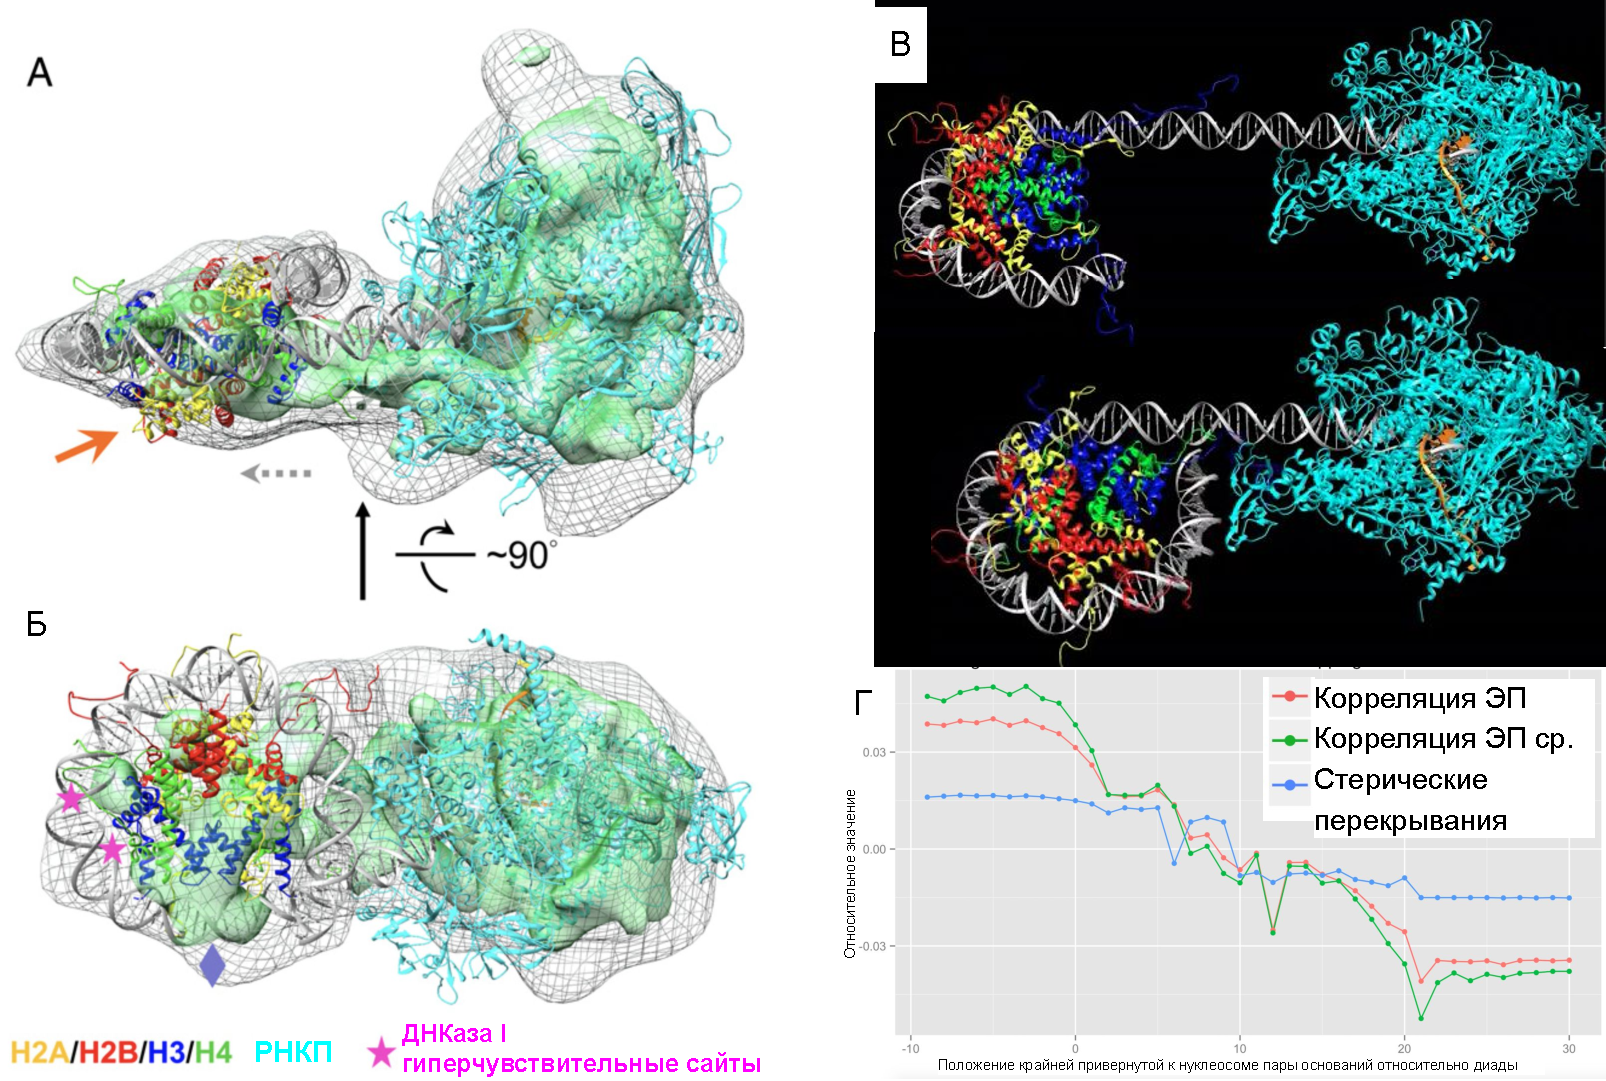
\includegraphics[width=\textwidth]{images/p6/p6_2/p6_2_pnas_f6.pdf}
    \caption[Структура комплекса элонгации остановленного в положении +42 нуклеосомы.]{Структура комплекса элонгации остановленного в положении +42 нуклеосомы. (A) Модель ЭК +42, построенная путем подбора оптимальной структуры комплекса, вписывающейся в электронную плотность, полученную экспериментально. Изоповерхность трехмерной реконструкции электронной плотности показана с более высоким или низким порогом серой сеткой или зеленым цветом, соответственно. Серая пунктирная и оранжевая стрелки указывают направление транскрипции и промотор-проксимальный димер H2A / H2B, экспонированный в раствор, соответственно. (Б) Структура была повернута на 90$^\circ$ вокруг горизонтальной оси. Положение участков ДНК, гиперчувствительных к ДНКазе I, показано звездочками. Нуклеосомная диада обозначена фиолетовым ромбом. (В) Различные варианты модели, отличиющиеся отворотом ДНК. (Г) График корелляции плотности модели и экспериментальной электронной плотности.}
    \label{fig:p6_2_pnas_f6}
\end{figure}
   
   
   Спейсер ДНК в полученной модели, соединяющий нуклеосому и РНКП, в значительной степени скрыт белками; таким образом структура согласуется с данными футпринтинга ДНКазы I, не обнаруживающими доступности спейсерной ДНК. Плотная структура комплекса согласуется с предположением, что у остановленного комлекса откат полимеразы сопровождается прикручиванием нуклеосомной ДНК к поверхности октамера гистонов. Докинг структуры элонгационного комплекса дрожжей Pol II в полученную модель свидетельствует о том, что подобный комплекс может быть образован эукариотический Pol II.
    
    Самая яркая и удивительная особенность комплекса +42 - это экспонирование поверхности промотор-проксимального димера гистонов H2A/H2B, взаимодействующего с ДНК. Действительно, модель +42 комплекса (рис. \ref{fig:p6_2_pnas_f6}) предполагает, что проксимальный участок H2A / H2B димера не стабилизируется взаимодействием с ДНК или РНКП, но остается связанным с октамером. Кроме того, наши предыдущие данные показали, что переход от комплекса +42 к +49 сопровождается полным приворотом нуклеосомной ДНК обратно на поверхность димера \cite{kulaeva_mechanism_2009}, предполагая, что димер не покидает ДНК до того, как Pol II продвинется более чем на 49 п.н. в нуклеосому. Стабильность димера во время транскрипции примечательна, учитывая, что октамер, свободный от ДНК, полностью теряет оба димера H2A / H2B менее, чем за 1 с \cite{feng_lifetime_1993}. Таким образом наличие нуклеосомной ДНК, которая остается частично накрученной вокруг тетрамера H3/H4 и промотор-дистального димера H2A/H2B приводит к снижению скорости диссоциации промотор-проксимального димера. Данные свидетельствуют о том, что связывание промотор - проксимального димера H2A/H2B с тетрамером H3/H4 в +42 комплексе может быть аллостерически стабилизировано оставшимися ДНК-гистоновыми взаимодействиями в нуклеосоме. Поскольку смещение димера представляет собой первый шаг к вытеснению всего октамера гистонов \cite{bintu_elongation_2011}, этот механизм, вероятно, важен для выживания нуклеосом во время различных процессов, включая ремоделирование нуклеосом.
    
    
    
   
    
\subsubsection{Обсуждение}
%2S дать красный текст pnas2015
    
    Наши данные идентифицируют переход из положения +48 в положение +49 как ключевой этап транскрипции через нуклеосому, где Pol II делает выбор между остановкой и дальнейшей транскрипцией. В минимальной системе, содержащей только Pol II и нуклеосому, этот выбор продиктован прежде всего последовательностью нуклеосомной ДНК, определяющей сродство ДНК-гистоновых взаимодействий и вероятность возврата Pol II. Особенно, Последовательность ДНК в области +(99–102) имеет решающее значение для выхода из положения +48.
    
    После преодоления нуклеосомного барьера в дальнейшем Pol II транскрипция обычно сопровождается выживанием нуклеосом благодаря образованию небольшой внутринуклеосомной петли ДНК на поверхности октамера гистонов. Высокая эффективность выживания нуклеосом оставалось загадкой, потому что транскрипция различными РНК-полимеразами сопровождается разворачиванием протяженного участка ДНК (до 80 п.н.) от октамера \cite{kulaeva_mechanism_2009,chang_structural_2013,bednar_nature_1999}, который, как ожидается, вызовет немедленную потерю димера H2A/H2B \cite{feng_lifetime_1993}. Наблюдаемая стабильность +42 комплекса, содержащего димер H2A / H2B, который экспонируется в растворитель свидетельствует о том, что связывание димера H2A/H2B с тетрамером H3/H4 может быть стабилизировано аллостерически и дает объяснение замечательной стабильность структуры нуклеосом во время различных процессов, включая транскрипцию \cite{kulaeva_mechanism_2009}, репликацию \cite{randall_fate_1992} и АТФ-зависимое ремоделирование хроматина \cite{mueller-planitz_nucleosome_2013}. Хотя один димер конститутивно вытесняется из нуклеосом при транскрипции \textit{in vitro} \cite{kireeva_nucleosome_2002}, это вытеснение, вероятно, происходит после транскрипции через позицию +49, поскольку ЭК+49 содержит оба димера H2A/H2B \cite{churchman_nascent_2011}.
    
    Описанная здесь паузирование в положениях +42/48 наблюдается у \textit{Drosophila} \cite{weber_nucleosomes_2014} и дрожжей \cite{churchman_nascent_2011}. В дрожжах первичный нуклеосомный барьер во время удлинения транскрипта  Pol II встречается, когда активный центр фермента находится в области +(40–55) п.н. в нуклеосоме . С аналогичным барьером сталкивается Pol II у дрозофилы во время транскрипции через нуклеосомы, локализованные на расстоянии более $\sim$400 п.н. от сайтов старта транскрипции \cite{weber_nucleosomes_2014}. Однако существуют дополнительные нуклеосомные барьеры в позициях -7 и +20 п.н. у Drosophila, характерные для нуклеосом, локализованные сразу после сайта старта транскрипции \cite{weber_nucleosomes_2014}.
    
    Недавние исследования показывают, что плотность комплексов Pol II вдоль транскрибированных генов, вероятно, определяет важные параметры транскрипции через хроматин - высоты нуклеосомных барьеров \cite{kulaeva_rna_2010,jin_synergistic_2010,chang_analysis_2014}, степень смещения гистонов и их обмен \cite{lee_evidence_2004,kulaeva_rna_2010,dion_dynamics_2007,rufiange_genome-wide_2007}. В то же время множественные факторы, включая модификации гистонов, варианты гистонов, шапероны гистонов и ремоделеры хроматина, дополнительно изменяют динамику гистонов на транскрибируемых генах \cite{smolle_resetting_2013,das_histone_2013,zentner_regulation_2013,weber_histone_2014}. Некоторые из эти факторов взаимодействуют с опухолевыми супрессорами \cite{wen_zmynd11_2014} и представляют важные мишени для разработки противоопухолевых препаратов \cite{garcia_facilitates_2013}.
    
    
    
    
    
    
    
    
    
    
    
    
    
    
    
    
    
    
    
    
    
    
    
    
    